\documentclass{article}
\usepackage{geometry}
\usepackage[utf8]{inputenc}
\usepackage{xcolor}
\usepackage{graphicx}
\usepackage{float,lscape}
\usepackage{listings}
\usepackage{color}
\usepackage{lipsum}% Used for dummy text.
\definecolor{titlepagecolor}{cmyk}{1,.60,0,.40}
\definecolor{namecolor}{cmyk}{1,.50,0,.10}
\definecolor{dkgreen}{rgb}{0,0.6,0}
\definecolor{gray}{rgb}{0.5,0.5,0.5}
\definecolor{mauve}{rgb}{0.58,0,0.82}
\lstset{frame=tb,
  language=Java,
  aboveskip=3mm,
  belowskip=3mm,
  showstringspaces=false,
  columns=flexible,
  basicstyle={\small\ttfamily},
  numbers=none,
  numberstyle=\tiny\color{gray},
  keywordstyle=\color{blue},
  commentstyle=\color{dkgreen},
  stringstyle=\color{mauve},
  breaklines=true,
  breakatwhitespace=true,
  tabsize=3
}
\title{Effective Field Method at Zero Temperature with Field Along Various Directions}
\author{Andrew Way}
\date{June 25th 2016}
%-----------------------------------------------------------------
\renewcommand{\topfraction}{.85}
\renewcommand{\bottomfraction}{.7}
\renewcommand{\textfraction}{.15}
\renewcommand{\floatpagefraction}{.66}
\renewcommand{\dbltopfraction}{.66}
\renewcommand{\dblfloatpagefraction}{.66}
\setcounter{topnumber}{9}
\setcounter{bottomnumber}{9}
\setcounter{totalnumber}{20}
\setcounter{dbltopnumber}{9}
\begin{document}

\maketitle

\tableofcontents

\clearpage
\section{Introduction}
    The effective field method was used to 3000 iterations (except where noted) to determine the 0 temperature states of 
    the 12x12x12 3D FCC kagome lattice while being subjected to a changing magnetic field along various field
    directions. 
    
    For several of these directions, the field was also decreased. Additionally, for several of these
    field directions, randomly generated lattices were also used as the starting configuration of the EFM simulation. The
    ground state used as the initial configuration in all ground state simulations had characteristic angles theta = 0.206275 and phi = 3.11867.
    
    The purpose of these simulations was to determine the dependence of the switching field on the field direction.
    Analysis that was performed on the resulting data included the following:
    \begin{itemize}
     \item Plots of magnetization versus field
     \item Plots of energy versus field
     \item Animations of the characteristic 6 spins 
     \item Determination of the number of ``unique'' spins that populate the lattice
     \item Determination of the components of the unique spins
     \item Dot products of each of the 6 spins with their respective $``neighbors''$.  
    \end{itemize}
\clearpage
\section{(001) Increasing Field, Ground State}
\paragraph
\large
The 6 spins begin to transition to the planar state at H=0.0105 and achieves the planar state at H=0.0121.
The pink and brown spins swap positions, as do the blue and purple spins, as the field increase beyond the planar state. 
The spins gradually align with the 001 field direction, until approximately at 0.14 the lattice becomes saturated and
the red and green and spins become parallel to the field direction. 
\begin{figure}[ht]
\centering
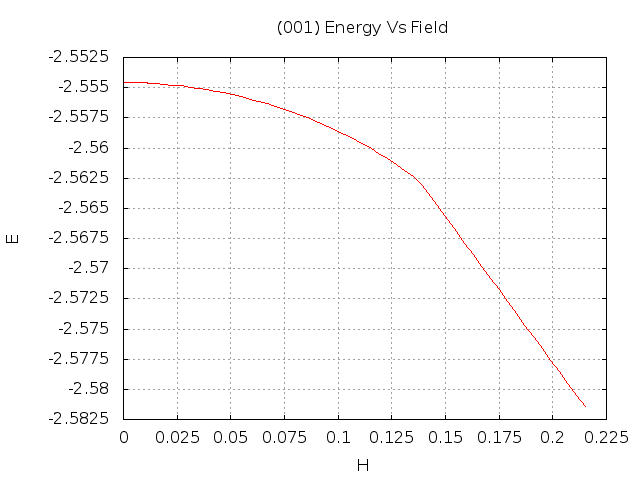
\includegraphics[scale=0.3]{HVariedData/Increasing/001Einc.png}
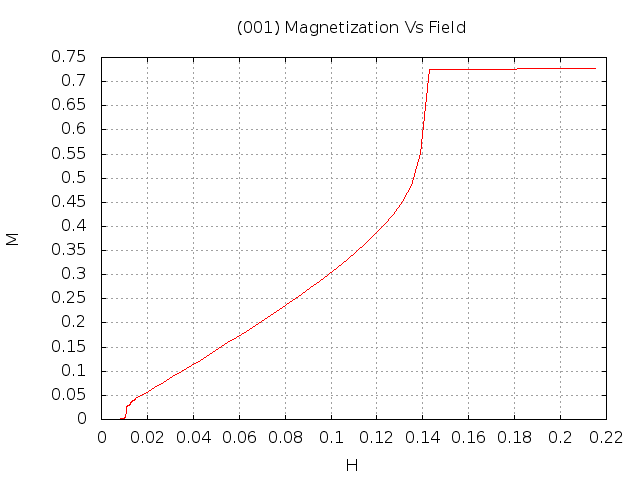
\includegraphics[scale=0.3]{HVariedData/Increasing/001Minc.png}
\end{figure}
\begin{figure}[ht]
\centering
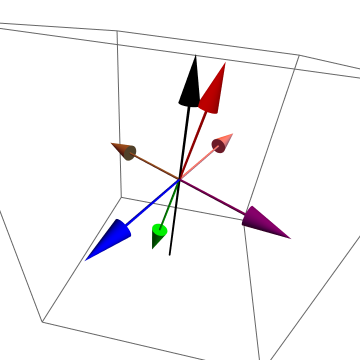
\includegraphics[scale=0.3]{HVariedData/Pictures/001Inc1.png}
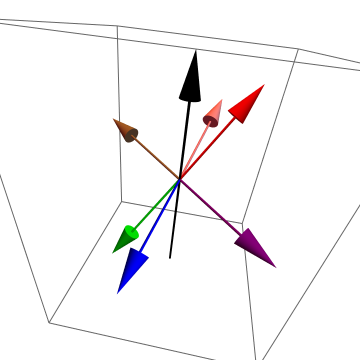
\includegraphics[scale=0.3]{HVariedData/Pictures/001Inc106.png}
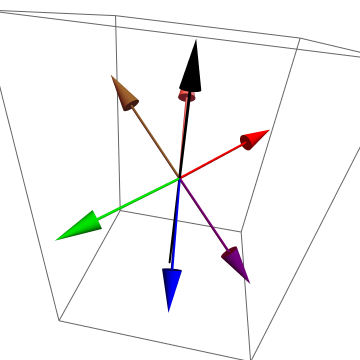
\includegraphics[scale=0.3]{HVariedData/Pictures/001Inc122.png}
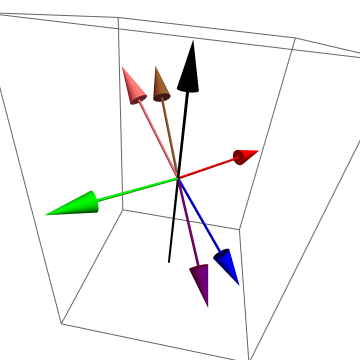
\includegraphics[scale=0.3]{HVariedData/Pictures/001Inc151.png}
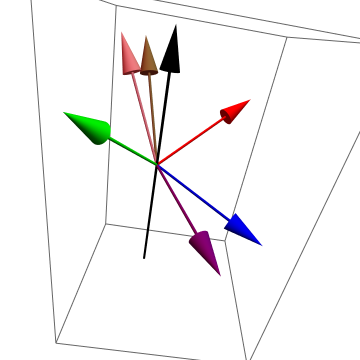
\includegraphics[scale=0.3]{HVariedData/Pictures/001Inc30S.png}
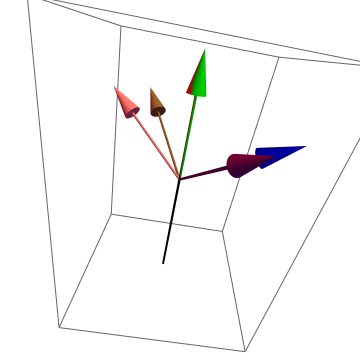
\includegraphics[scale=0.3]{HVariedData/Pictures/001Inc35S.png}
\caption{Snap shots of the 6 characteristic spins at H=0, 0.0105, 0.0121, 0.0150, 0.131, 0.151. The black arrow
indicates the direction of the field. \textbf{Note}: In all 6-spin snapshots, the spins are as such: A-Red, B-Green, C-Blue, D-Pink, E-Brown, F-Purple}
\end{figure}

\clearpage

\section{(001) Decreasing Field, Ground State}
\paragraph
\large
The lattice leaves the saturated state at a field lower than what was required to induce it while increasing the field.
This transition from saturation occurs at approximately H=0.13, compared to the transition to saturation at H=0.14 when increasing the field. %Description here
The spins gradually unalign and rest in a planar state at zero field, and is characterized by the groundstate angles ADD HERE
\begin{figure}[ht]
\centering
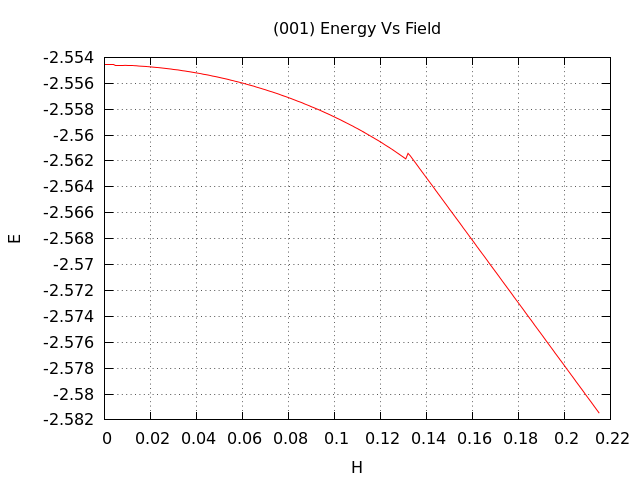
\includegraphics[scale=0.3]{HVariedData/Decreasing/001Edec.png}
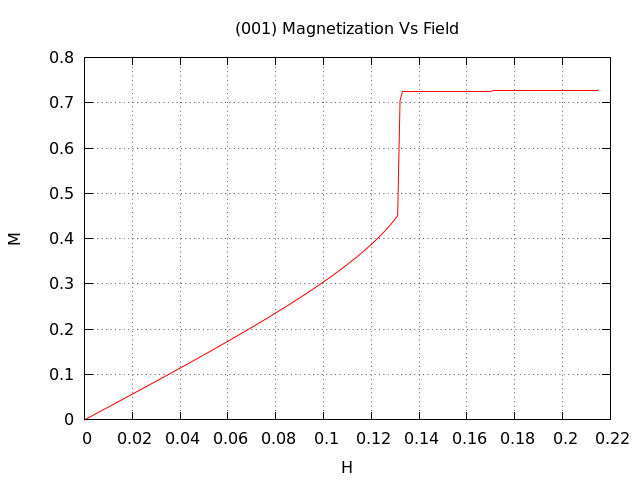
\includegraphics[scale=0.3]{HVariedData/Decreasing/001Mdec.png}
\end{figure}
\begin{figure}[ht]
\centering
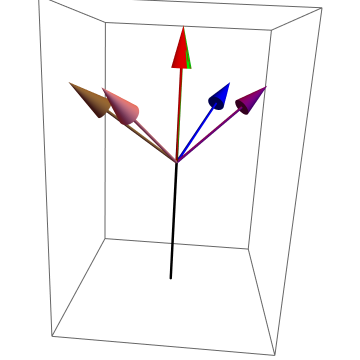
\includegraphics[scale=0.37]{HVariedData/Pictures/001Dec1.png}
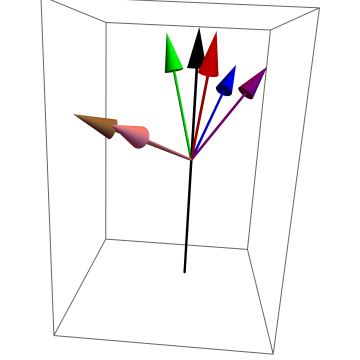
\includegraphics[scale=0.37]{HVariedData/Pictures/001Dec84.png}
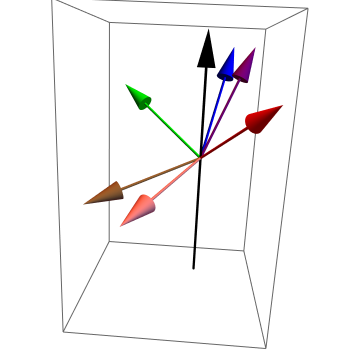
\includegraphics[scale=0.37]{HVariedData/Pictures/001Dec86.png}
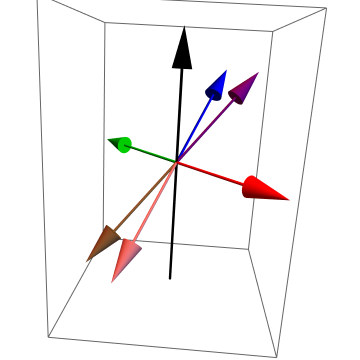
\includegraphics[scale=0.37]{HVariedData/Pictures/001Dec216.png}
\caption{Snapshots at H=0.215, 0.132, 0.130, 0}
\end{figure}

\begin{center}
\begin{figure}
\centering
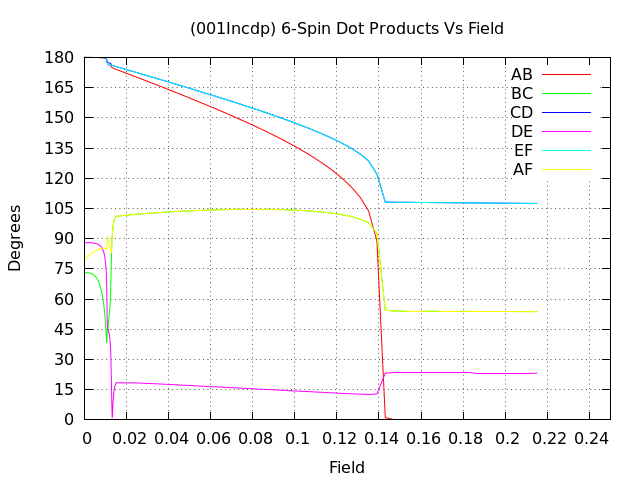
\includegraphics[scale=0.55]{HVariedData/Pictures/001Incdp.png}
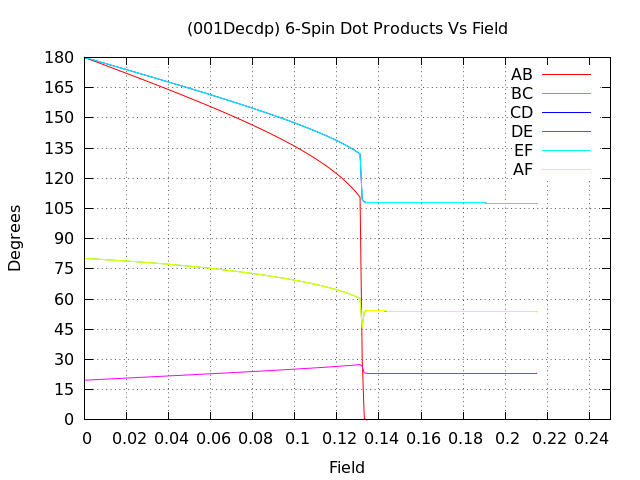
\includegraphics[scale=0.55]{HVariedData/Pictures/001Decdp.png}
\caption{Dot products between the characteristic spins for both increasing and decreasing field.}
\end{figure}
\end{center}

\begin{figure}[ht]
\centering
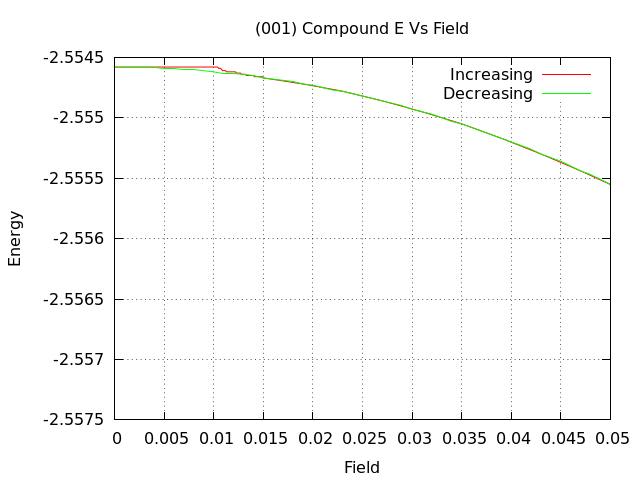
\includegraphics[scale=0.6]{HVariedData/compoundEM/001Ecompound.png}
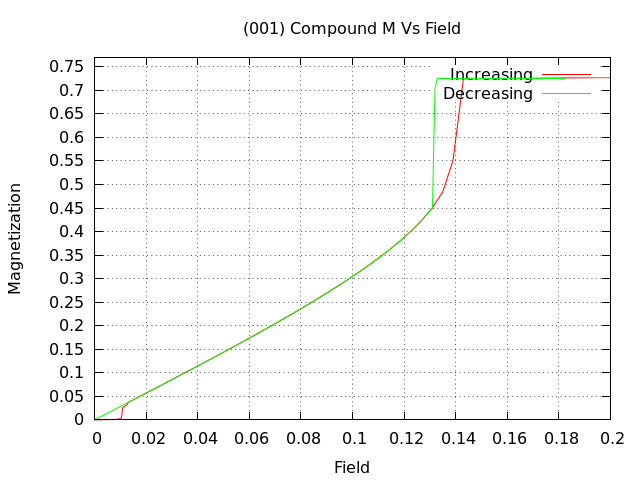
\includegraphics[scale=0.6]{HVariedData/compoundEM/001Mcompound.png}
\caption{Composite graphs of energy and magnetization for both decreasing and increasing field magnitude.}
\end{figure}
\clearpage

\section{(010) Increasing Field, Ground State}
\paragraph
\large
The lattice begins to undergo a transition at 0.0110. At 0.0114 the planar state is achieved. Similar to 001,
two pairs of spins begin to swap positions at around 0.015, though the pairs consist of spins different from 001.
The blue and green spins and red and pink spins appear to be swapping positions, but never do. The spins gradually
align with the 010 direction until at approximately H=0.14 the lattice becomes saturated and the purple and brown spins
become parallel to the field direction.%Description here

\begin{figure}[ht]
\centering
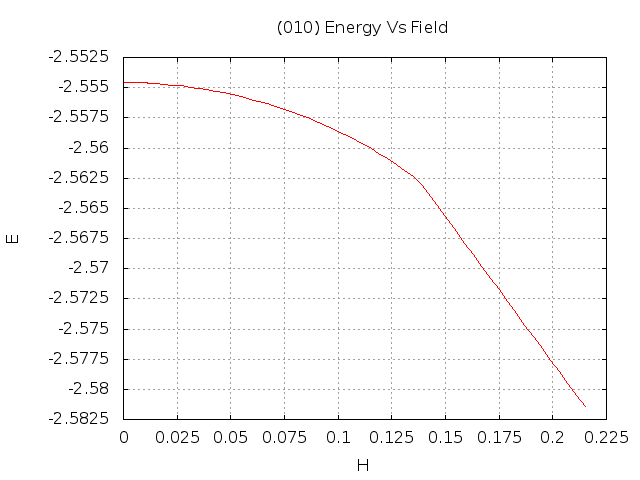
\includegraphics[scale=0.3]{HVariedData/Increasing/010Einc.png}
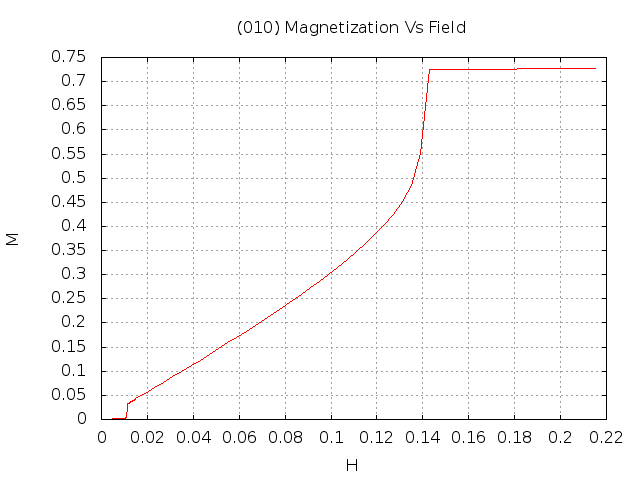
\includegraphics[scale=0.3]{HVariedData/Increasing/010Minc.png}
\end{figure}
\begin{figure}[ht]
\centering
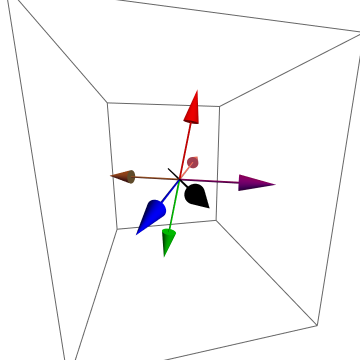
\includegraphics[scale=0.3]{HVariedData/Pictures/010Inc1.png}
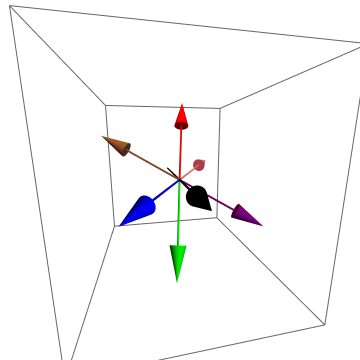
\includegraphics[scale=0.3]{HVariedData/Pictures/010Inc111.png}
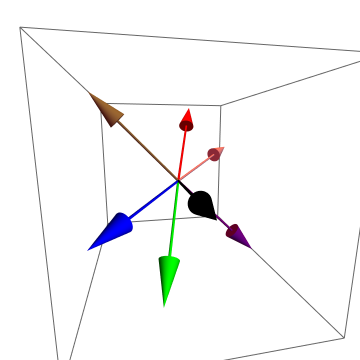
\includegraphics[scale=0.3]{HVariedData/Pictures/010Inc118.png}
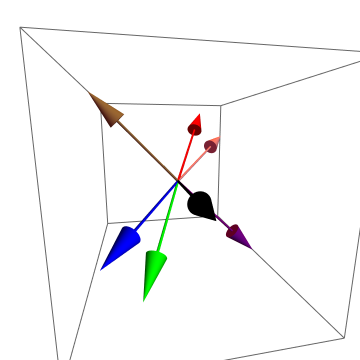
\includegraphics[scale=0.3]{HVariedData/Pictures/010Inc151.png}
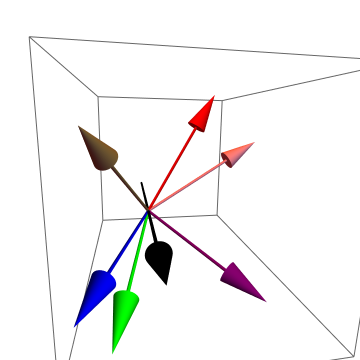
\includegraphics[scale=0.3]{HVariedData/Pictures/010Inc32S.png}
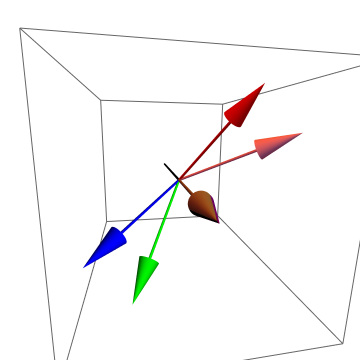
\includegraphics[scale=0.3]{HVariedData/Pictures/010Inc33S.png}
\caption{Snapshots at H=0, 0.0110, 0.0117, 0.0150, 0.139, 0.179 }
\end{figure}

\clearpage

\section{(010) Decreasing Field, Ground State}
\paragraph
\large
The lattice is released from saturation at approximately field=0.13, a field magnitude lower than the increasing field required
to induce saturation. The spins gradually unalign with the decreasing field, and rest at a zero field planar state
characterized by angles ADD HERE%Description here

\begin{figure}[ht]
\centering
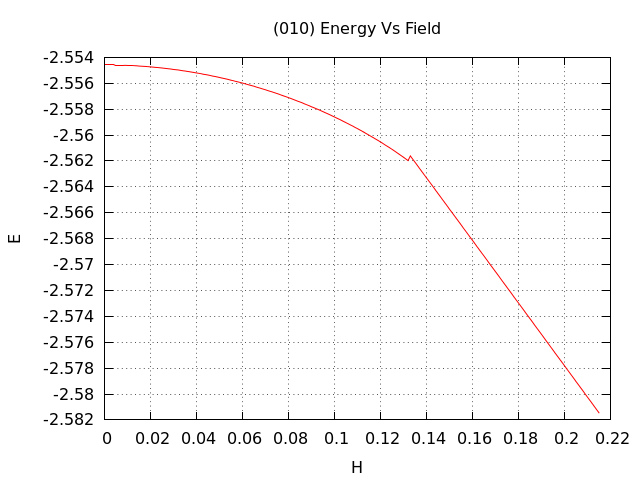
\includegraphics[scale=0.3]{HVariedData/Decreasing/010Edec.png}
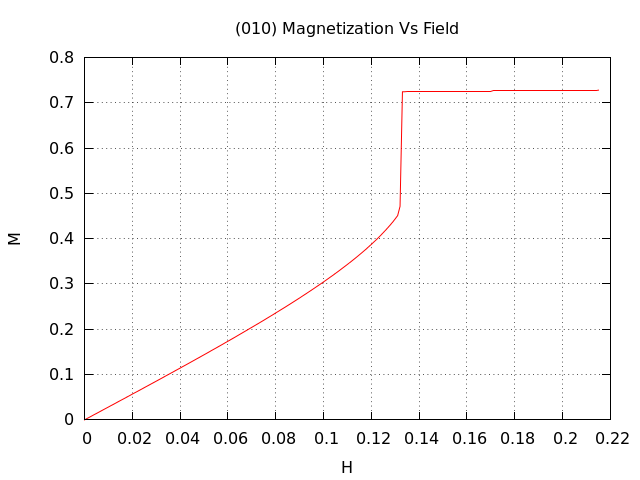
\includegraphics[scale=0.3]{HVariedData/Decreasing/010Mdec.png}
\end{figure}
\begin{figure}[ht]
\centering
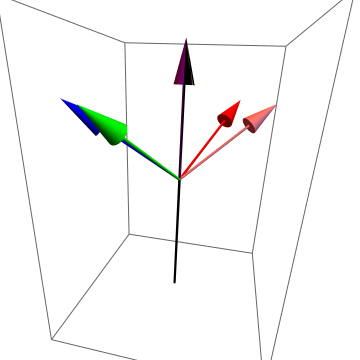
\includegraphics[scale=0.37]{HVariedData/Pictures/010Dec1.png}
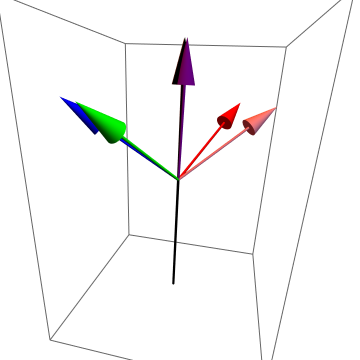
\includegraphics[scale=0.37]{HVariedData/Pictures/010Dec83.png}
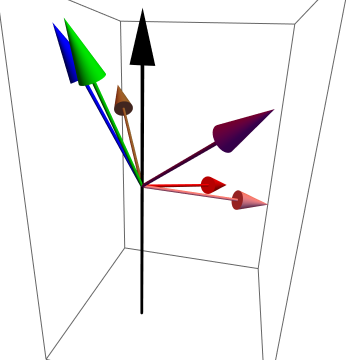
\includegraphics[scale=0.37]{HVariedData/Pictures/010Dec84.png}
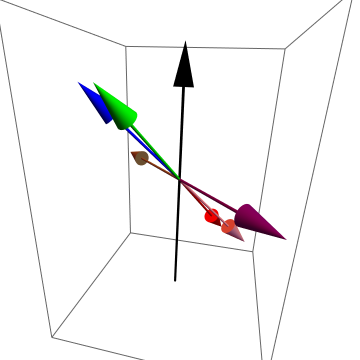
\includegraphics[scale=0.37]{HVariedData/Pictures/010Dec216.png}
\caption{Snapshots of the 6 characteristic spins at H=0.215, 0.132, 0.131, 0}
\end{figure}

\begin{center}
\begin{figure}
\centering
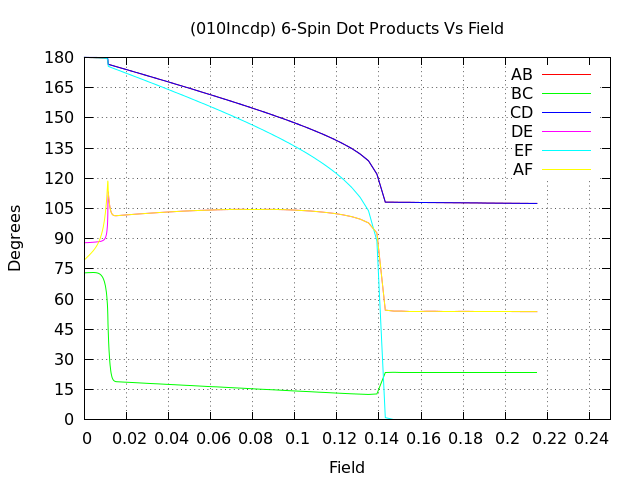
\includegraphics[scale=0.5]{HVariedData/Pictures/010Incdp.png}
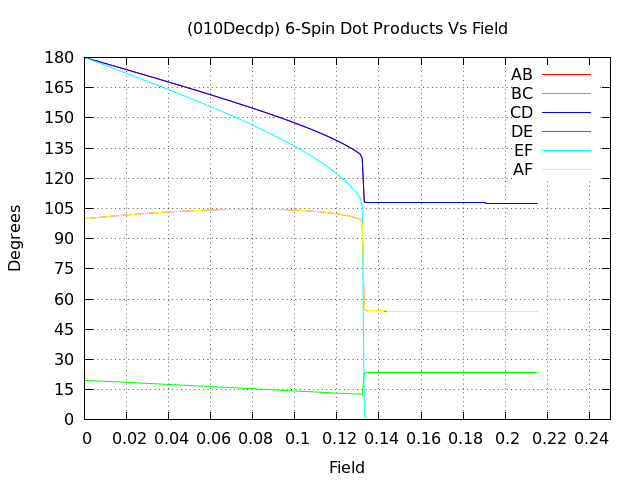
\includegraphics[scale=0.5]{HVariedData/Pictures/010Decdp.png}
\caption{Dot products between the characteristic spins for both increasing and decreasing field.}
\end{figure}
\end{center}
\clearpage
\begin{figure}[ht]
\centering
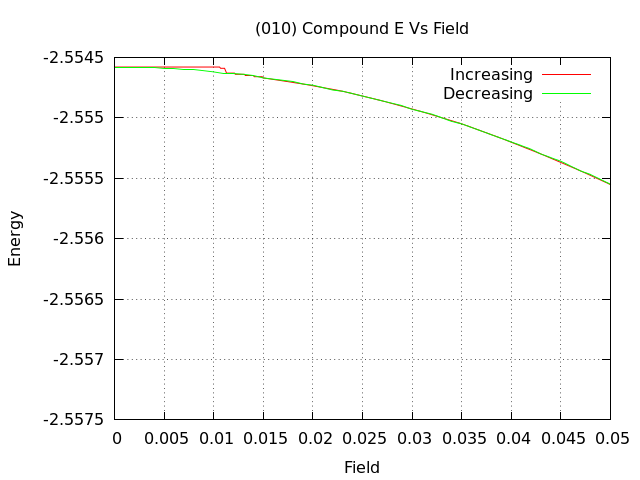
\includegraphics[scale=0.6]{HVariedData/compoundEM/010Ecompound.png}
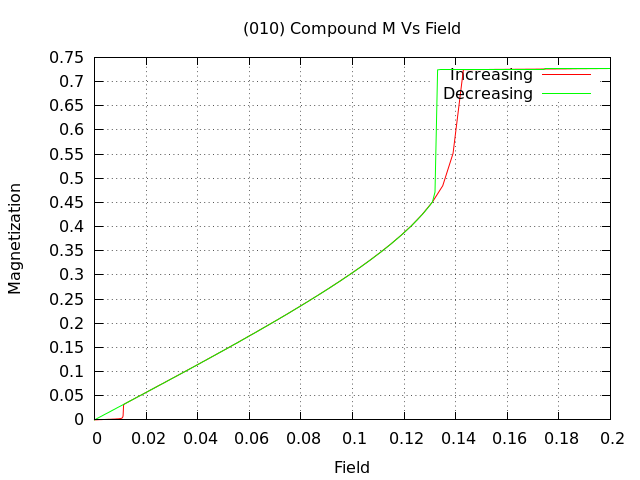
\includegraphics[scale=0.6]{HVariedData/compoundEM/010Mcompound.png}
\caption{Composite graphs of energy and magnetization for both decreasing and increasing field magnitude.}
\end{figure}
\clearpage
\section{(011) Increasing Field, Ground State}
\paragraph
\large
The lattice begins to transition at approximately 0.007. At 0.0074 the planar state is achieved. At 0.0093, the 
pink and red spins swap position, and the blue and green spins swap position. As the field is increased further to 0.0115,
the green and brown spins begin to swap positions. At 0.143, this is achieved. Once saturated, no spins are parallel
with the field direction.%Description here

\begin{figure}[ht]
\centering
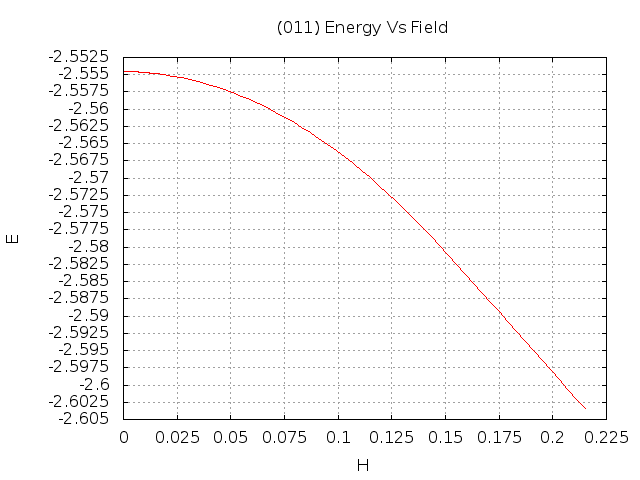
\includegraphics[scale=0.3]{HVariedData/Increasing/011Einc.png}
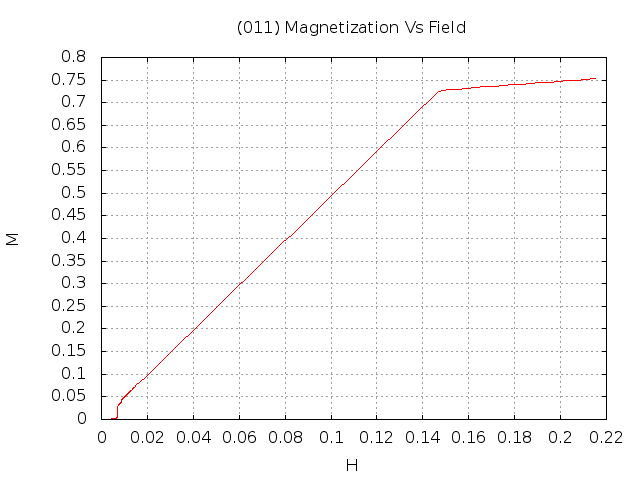
\includegraphics[scale=0.3]{HVariedData/Increasing/011Minc.png}
\end{figure}
\begin{figure}[ht]
\centering
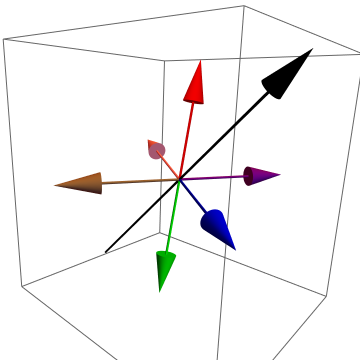
\includegraphics[scale=0.3]{HVariedData/Pictures/011Inc1.png}
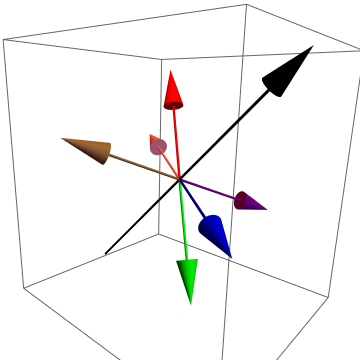
\includegraphics[scale=0.3]{HVariedData/Pictures/011Inc67.png}
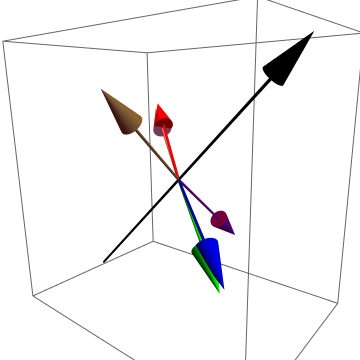
\includegraphics[scale=0.3]{HVariedData/Pictures/011Inc82.png}
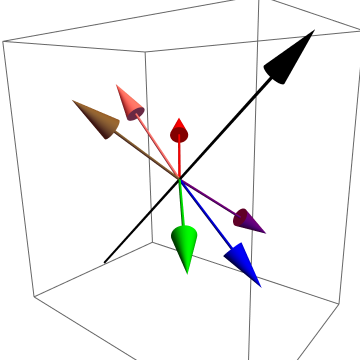
\includegraphics[scale=0.3]{HVariedData/Pictures/011Inc94.png}
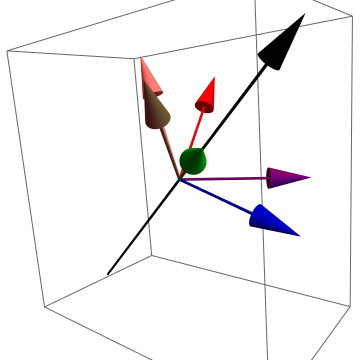
\includegraphics[scale=0.3]{HVariedData/Pictures/011Inc26S.png}
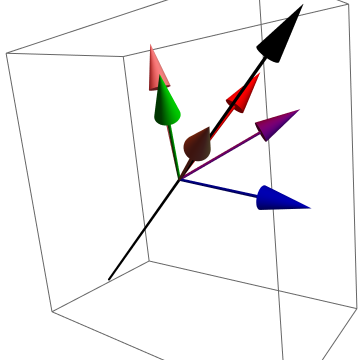
\includegraphics[scale=0.3]{HVariedData/Pictures/011Inc39S.png}
\caption{Snapshots at H=0, 0.0066, 0.0082, 0.0094, 0.115, 0.167}
\end{figure}

\clearpage

\section{(011) Decreasing Field, Ground State}
\paragraph
\large
As the field is decreased to 0.134, the brown and green spins swap positions again. All 6 spins gradually unalign
with the field until they reach a zero field planar state characterized by angles ADD HERE%Description here

\begin{figure}[ht]
\centering
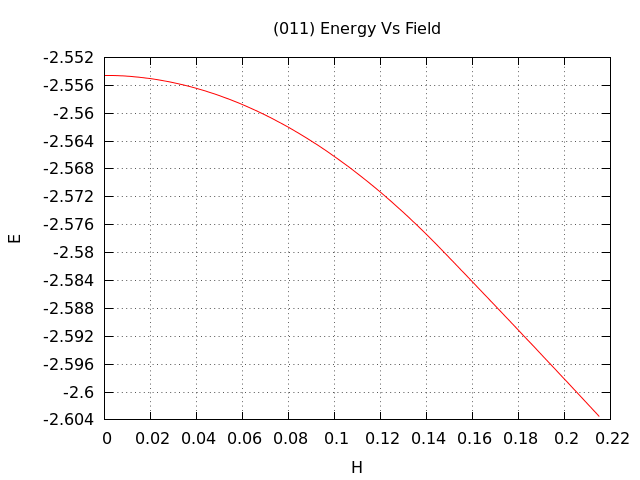
\includegraphics[scale=0.3]{HVariedData/Decreasing/011Edec.png}
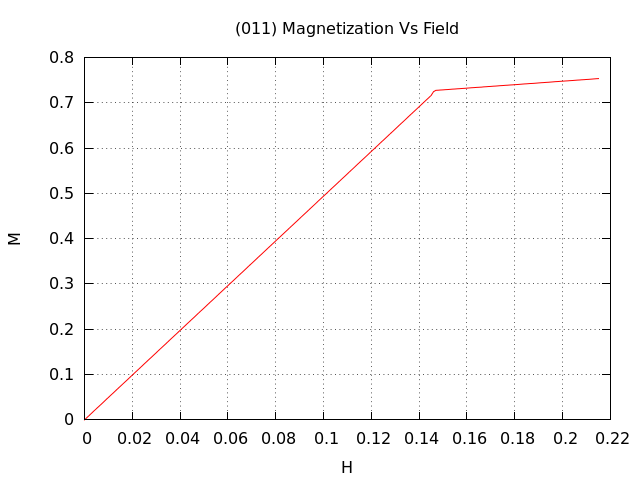
\includegraphics[scale=0.3]{HVariedData/Decreasing/011Mdec.png}
\end{figure}
\begin{figure}[ht]
\centering
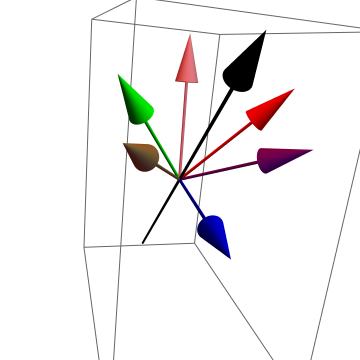
\includegraphics[scale=0.37]{HVariedData/Pictures/011Dec1.png}
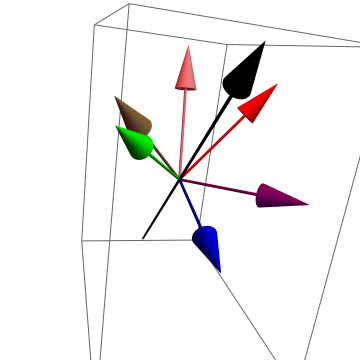
\includegraphics[scale=0.37]{HVariedData/Pictures/011Dec82.png}
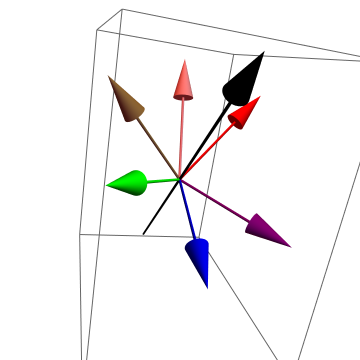
\includegraphics[scale=0.37]{HVariedData/Pictures/011Dec122.png}
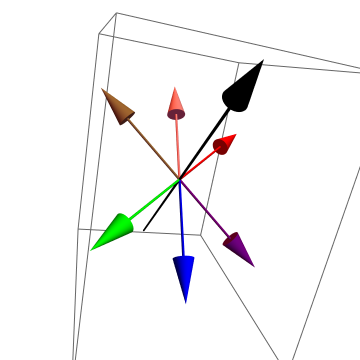
\includegraphics[scale=0.37]{HVariedData/Pictures/011Dec216.png}
\caption{Snapshots at H=0.215, 0.134, 0.094, 0}
\end{figure}

\begin{center}
\begin{figure}
\centering
\includegraphics[scale=0.5]{HVariedData/Pictures/011Incdp.png}
\includegraphics[scale=0.5]{HVariedData/Pictures/011Decdp.png}
\caption{Dot products between the characteristic spins for both increasing and decreasing field.}
\end{figure}
\end{center}
\clearpage

\begin{figure}[ht]
\centering
\includegraphics[scale=0.6]{HVariedData/compoundEM/011Ecompound.png}
\includegraphics[scale=0.6]{HVariedData/compoundEM/011Mcompound.png}
\caption{Composite graphs of energy and magnetization for both decreasing and increasing field magnitude.}
\end{figure}
\clearpage
\section{(100) Increasing Field, Ground State}
\paragraph
\large
%\addcontentsline{toc}{section}{Unnumbered Section}
Two inflection points are observed in the magnetization graph. There are two inflection points in the
energy graph as well, however they are not as obvious. A planar state is achieved at 0.0041. Between 0.0041 and
0.0064, the brown and green spins become closer to one another, as do the red and purple spins. The pink and blue
spins remain fixed. The spins gradually align with the field, until it suddenly snaps into its final position where
the blue and pink spins point in the same direction, in addition to lying within the xy plane. The lattice is
saturated beyond this point. 
\begin{figure}[h]
 \centering 
\includegraphics[scale=0.3]{100/E000to005G.png}
\includegraphics[scale=0.3]{100/M000to005G.png}
\caption{Energy vs increasing field and Magnetization versus increasing field}
\end{figure}
\begin{figure}[ht]
\centering
\includegraphics[scale=0.28]{100/1S000to005G.png}
\includegraphics[scale=0.28]{100/39S000to005G.png}
\includegraphics[scale=0.28]{100/42S000to005G.png}
\includegraphics[scale=0.28]{100/55S000to005G.png}
\includegraphics[scale=0.28]{100/419S000to005G.png}
\includegraphics[scale=0.28]{100/466S000to005G.png}
\includegraphics[scale=0.28]{100/467S000to005G.png}
\includegraphics[scale=0.28]{100/501S000to005G.png}
\caption{H=0, 0.0038, 0.0041, 0.0054, 0.0418, 0.0465, 0.0466 and 0.05}
\end{figure}

\clearpage
\section{(100) Decreasing Field, Ground State}
\paragraph
\large
As the field is decreased, the spins are released from the saturated state, and return to the typically observed
planar state, that gradually unaligns with the field direction as the field is decreased. Finally, the spins return
to a full planar state, and not the original zero field ground state. The starting configuration of this run
was not the final configuration of the (100) Increasing Field, Ground State run, but the same zero field ground state
that the (100) Increasing Field, Ground state started from. This is the case for all Ground State runs, except where
noted. 
\begin{figure}[ht]
 \centering 
\includegraphics[scale=0.3]{100/E005to000G.png}
\includegraphics[scale=0.3]{100/M005to000G.png}
\caption{Energy vs decreasing field and Magnetization versus decreasing field}
\end{figure}
\begin{figure}[ht]
\centering
\includegraphics[scale=0.27]{100/1S005to000G.png}
\includegraphics[scale=0.27]{100/3S005to000G.png}
\includegraphics[scale=0.27]{100/55S005to000G.png}
\includegraphics[scale=0.27]{100/56S005to000G.png}
\includegraphics[scale=0.27]{100/129S005to000G.png}
\includegraphics[scale=0.27]{100/501S005to000G.png}
\caption{H=0.05, 0.0498, 0.0446, 0.0445, 0.0372, and 0. It can be seen that the pink and blue spins have not yet
entirely lined up with the field vector in the first picture, but they have in the second picture. This indicates that
simply using a zero field groundstate and subjecting it to a high field immediately with only 3000 steps does not yield
the true state for that field.}
\end{figure}
\clearpage

\begin{figure}[ht]
\centering
\includegraphics[scale=0.5]{HVariedData/Pictures/100Decdp.png}
\includegraphics[scale=0.5]{HVariedData/Pictures/100Incdp.png}
\caption{Dot products between the characteristic spins for both increasing and decreasing field. The data only continues
to a low field relative to other simulations due to the saturation field occuring so early. A simulation continuing
this run is currently being worked on.}
\end{figure}
\clearpage

\begin{figure}[ht]
\centering
\includegraphics[scale=0.6]{HVariedData/compoundEM/100Ecompound.png}
\includegraphics[scale=0.6]{HVariedData/compoundEM/100Mcompound.png}
\caption{Composite graphs of energy and magnetization for both decreasing and increasing field magnitude.}
\end{figure}
\clearpage

\begin{figure}[ht]
\centering
\includegraphics[scale=0.5]{100/000to005Freq.png}
\includegraphics[scale=0.5]{100/005to000Freq.png}
\caption{(100 Decreasing Field, Ground state) Dot products of each spin with its neighbours. The number of unique spins within the lattice is also present.}
\end{figure}
\clearpage

\section{(100) Increasing Field, Random State}
The energy drops very quickly at near zero field, which is likely because of insufficient number of iterations. Two
points of inflection are observed. The transition of the spins is very similar to starting from a ground state.
\begin{figure}[h]
 \centering 
\includegraphics[scale=0.3]{100/E000to005R.png}
\includegraphics[scale=0.3]{100/M000to005R.png}
\caption{Energy vs increasing field and Magnetization versus increasing field}
\end{figure}
\begin{figure}[ht]
\centering
\includegraphics[scale=0.27]{100/1S000to005R.png}
\includegraphics[scale=0.27]{100/2S000to005R.png}
\includegraphics[scale=0.27]{100/48S000to005R.png}
\includegraphics[scale=0.27]{100/54S000to005R.png}
\includegraphics[scale=0.27]{100/55S000to005R.png}
\includegraphics[scale=0.27]{100/411S000to005R.png}
\includegraphics[scale=0.27]{100/467S000to005R.png}
\includegraphics[scale=0.27]{100/501S000to005R.png}
\caption{H = 0.00, 0.0001, 0.0047, 0.0053, 0.0054, 0.0410, 0.0466, 0.05}
\end{figure}
\clearpage

\section{(100) Decreasing Field, Random State}
The lattice starts off in a planar state. As the field is decreased, spins gradually unalign with the field. 
Suddenly, at 0.0455, the spins snap back into a slight realigned planar state. Another sudden readjustment
is observed at 0.025. Finally, the spins return a full planar state at 0 field. The red and brown spins
swap positions as the field lowers, as do the green and purple spins. This is likely a result of insufficient EFM iterations.
\begin{figure}[h]
 \centering 
\includegraphics[scale=0.3]{100/E005to000R.png}
\includegraphics[scale=0.3]{100/M005to000R.png}
\caption{Energy vs decreasing field and Magnetization versus decreasing field}
\end{figure}
\begin{figure}[ht]
\centering
\includegraphics[scale=0.3]{100/1S005to000R.png}
\includegraphics[scale=0.3]{100/41S005to000R.png}
\includegraphics[scale=0.3]{100/46S005to000R.png}
\includegraphics[scale=0.3]{100/244S005to000R.png}
\includegraphics[scale=0.3]{100/245S005to000R.png}
\includegraphics[scale=0.3]{100/501S005to000R.png}
\caption{H = 0.05, 0.0460, 0.0455, 0.0257, 0.0256, 0.00.}
\end{figure}
\clearpage

\begin{figure}[ht]
\centering
\includegraphics[scale=0.5]{HVariedData/Pictures/100DecdpR.png}
\includegraphics[scale=0.5]{HVariedData/Pictures/100IncdpR.png}
\caption{Dot products between the characteristic spins for both increasing and decreasing field. The data only continues
to a low field relative to other simulations due to the saturation field occuring so early. A simulation continuing
this run is currently being worked on.}
\end{figure}
\clearpage


\begin{figure}[ht]
\centering
\includegraphics[scale=0.5]{100/000to005RFreq.png}
\includegraphics[scale=0.5]{100/005to000RFreq.png}
\caption{At high field, a huge number of $``unique''$ spins was observed. When looking through one of the configuration
files, most spins only agreed with some other spins to at most 1 decimal place. The program that determines whether
a spin is unique considers a spin to be unique when it doesn't agree with any previously found spin up to at least two decimal 
places. Hence, the large number of unique spins present.The plateau in the middle is actually just false data I put
into the text file, since I cancelled the program since it was taking a very long time. I reran the program from around
H = 0.0250 to 0, and found that the lattice in this field range always had 6 unique spins.}
\end{figure}
\clearpage
\section{(101) Increasing Field, Ground State}
\paragraph
\large
The lattice begins to undergo a transition to a planar state at 0.0055, where it is achieved at 0.0060. At 0.0115 
the purple and red spins and green and brown spins begin to swap positions, which is complete at 0.0128. At approximately
0.14, the green and pink spins swap position. Upon swapping, the lattice becomes saturated.%Description here

\begin{figure}[ht]
\centering
\includegraphics[scale=0.3]{HVariedData/Increasing/101Einc.png}
\includegraphics[scale=0.3]{HVariedData/Increasing/101Minc.png}
\end{figure}
\begin{figure}[ht]
\centering
\includegraphics[scale=0.29]{HVariedData/Pictures/101Inc1.png}
\includegraphics[scale=0.29]{HVariedData/Pictures/101Inc56.png}
\includegraphics[scale=0.29]{HVariedData/Pictures/101Inc61.png}
\includegraphics[scale=0.29]{HVariedData/Pictures/101Inc116.png}
\includegraphics[scale=0.29]{HVariedData/Pictures/101Inc128.png}
\includegraphics[scale=0.29]{HVariedData/Pictures/101Inc32S.png}
\includegraphics[scale=0.29]{HVariedData/Pictures/101Inc38S.png}
\caption{H=0, 0.0055, 0.0060, 0.0115, 0.0128, 0.0.139, 0.163}
\end{figure}
\clearpage

\section{(101) Decreasing Field, Ground State}
\paragraph
\large
When decreasing the field, instead of the pink and green re-swapping positions the
blue and red spins, the spins that mirror them, swap positions at approximately 0.137. %Description here
\begin{figure}[ht]
\centering
\includegraphics[scale=0.3]{HVariedData/Decreasing/101Edec.png}
\includegraphics[scale=0.3]{HVariedData/Decreasing/101Mdec.png}
\end{figure}
\begin{figure}[ht]
\centering
\includegraphics[scale=0.37]{HVariedData/Pictures/101Dec1.png}
\includegraphics[scale=0.37]{HVariedData/Pictures/101Dec79.png}
\includegraphics[scale=0.37]{HVariedData/Pictures/101Dec125.png}
\includegraphics[scale=0.37]{HVariedData/Pictures/101Dec216.png}
\caption{Snapshots at H=0.2150, 0.137, 0.09, 0}
\end{figure}

\begin{center}
\begin{figure}
\centering
\includegraphics[scale=0.5]{HVariedData/Pictures/101Incdp.png}
\includegraphics[scale=0.5]{HVariedData/Pictures/101Decdp.png}
\caption{Dot products between the characteristic spins for both increasing and decreasing field.}
\end{figure}
\end{center}
\clearpage

\begin{figure}[ht]
\centering
\includegraphics[scale=0.6]{HVariedData/compoundEM/101Ecompound.png}
\includegraphics[scale=0.6]{HVariedData/compoundEM/101Mcompound.png}
\caption{Composite graphs of energy and magnetization for both decreasing and increasing field magnitude.}
\end{figure}
\clearpage

%110 ----------------------------------------------------------------------------------------------
\pagebreak
\section{(110) Increasing Field, Ground State}
Two inflection points are evident in the graphs of energy and magnetization, indicating the occurence of a sudden
change in orientation of the spins. The first inflection point occurs at H~0.005, at which the spins snap into a 
planar state. The second occurs at H~0.009, where another planar state forms but oriented in a different direction. From 
thereon out, the spins gradually align with the 110 field and nothing else interesting happens. 
\begin{figure}[ht]
 \centering 
\includegraphics[scale=0.3]{110/E000to005G.png}
\includegraphics[scale=0.3]{110/M000to005G.png}
\caption{Energy vs increasing field and Magnetization versus increasing field}
\end{figure}
\begin{figure}[ht]
\centering
\includegraphics[scale=0.3]{110/1S000to005G.png}
\includegraphics[scale=0.3]{110/47S000to005G.png}
\includegraphics[scale=0.3]{110/50S000to005G.png}
\includegraphics[scale=0.3]{110/86S000to005G.png}
\includegraphics[scale=0.3]{110/96S000to005G.png}
\includegraphics[scale=0.3]{110/501S000to005G.png}
\caption{Snapshots of the 6 characteristic spins of the lattice at H=0, 0.0046, 0.0052, 0.0082, 0.0091, 0.0097, and 0.05}
\end{figure}
\clearpage

\begin{figure}[ht]
\centering
\includegraphics[scale=0.5]{110/000to005Freq.png}
\includegraphics[scale=0.5]{110/005to000Freq.png}
\caption{put text}
\end{figure}
\clearpage

\section{(110) Decreasing Field, Ground State}
Similar to starting with a high field in the 111 direction, the spins are in a planar state that is
aligned with the field. When the field is lowered, the spins are stuck in a planar state. In the first
snapshot of the spins, the brown and green spins are partially aligned. This is likely due to insufficient
number of iterations for EFM.
\begin{figure}[h]
 \centering 
\includegraphics[scale=0.3]{110/E005to000G.png}
\includegraphics[scale=0.3]{110/M005to000G.png}
\caption{Energy vs decreasing field and Magnetization versus decreasing field}
\end{figure}
\begin{figure}[ht]
\centering
\includegraphics[scale=0.32]{110/1S005to000G.png}
\includegraphics[scale=0.32]{110/2S005to000G.png}
\includegraphics[scale=0.32]{110/200S005to000G.png}
\includegraphics[scale=0.32]{110/501S005to000G.png}
\caption{Snapshots of the 6 characteristic spins of the lattice at B=0.05, B=0.0301, and B=0.00}
\end{figure}
\clearpage

\begin{figure}[ht]
\centering
\includegraphics[scale=0.5]{HVariedData/Pictures/110Incdp.png}
\includegraphics[scale=0.5]{HVariedData/Pictures/110Decdp.png}
\caption{put text}
\end{figure}
\clearpage

\begin{figure}[ht]
\centering
\includegraphics[scale=0.6]{HVariedData/compoundEM/110Ecompound.png}
\includegraphics[scale=0.6]{HVariedData/compoundEM/110Mcompound.png}
\caption{Composite graphs of energy and magnetization for both decreasing and increasing field magnitude.}
\end{figure}
\clearpage

\section{(110) Increasing Field, Random State}
Very similar to run 1, in that there are 2 transitions at approximately 0.0038 and 0.0075. The transformation of the 
6 spins is similar as well,
with the spins beginning in the groundstate, transition to a planar state, 2 pairs of spins rotate and switch places,
and the plane the spins lie in reorients itself. The spins then gradually align with the field, and nothing
else interesting happens. 
\begin{figure}[ht]
 \centering 
\includegraphics[scale=0.3]{110/E000to005R.png}
\includegraphics[scale=0.3]{110/M000to005R.png}
\caption{Energy vs increasing field and Magnetization versus increasing field}
\end{figure}
\begin{figure}[ht]
\centering
\includegraphics[scale=0.33]{110/1S000to005R.png}
\includegraphics[scale=0.33]{110/69S000to005R.png}
\includegraphics[scale=0.33]{110/82S000to005R.png}
\includegraphics[scale=0.33]{110/501S000to005R.png}
\caption{Snapshots of the 6 spins at H = 0.00, 0.0068, 0.0081, and 0.05}
\end{figure}
\clearpage

\begin{figure}[ht]
\centering
\includegraphics[scale=0.5]{110/000to005RFreq.png}
\includegraphics[scale=0.5]{110/005to000RFreq.png}
\caption{The lattice seems to be having trouble finding a stable 6 spin configuration. A sudden transition is observed
at approximately 0.028 field, which can be observed in all graphs from this simulation.}
\end{figure}
\clearpage

\section{(110) Decreasing Field, Random State}
A sudden transition occurs at approximately 0.022. The green and pink spins swap places with another, and the blue
and red spins also follow this swap. It's possible this transition only occurs because there is insufficient
steps being used for EFM, as was the case with applying the field in the 111 direction. Any transitions disappeared
when increasing the number of steps from 2000 to 3000 steps when decreasing the field with a random initial 
configuration. 
\begin{figure}[ht]
 \centering 
\includegraphics[scale=0.3]{110/E005to000R.png}
\includegraphics[scale=0.3]{110/M005to000R.png}
\caption{Energy vs decreasing field and Magnetization versus decreasing field}
\end{figure}
\begin{figure}[ht]
\centering
\includegraphics[scale=0.23]{110/1S005to000R.png}
\includegraphics[scale=0.23]{110/241S005to000R.png}
\includegraphics[scale=0.23]{110/300S005to000R.png}
\includegraphics[scale=0.23]{110/501S005to000R.png}
\caption{}
\end{figure}
\clearpage

\begin{figure}[ht]
\centering
\includegraphics[scale=0.5]{HVariedData/Pictures/110IncdpR.png}
\includegraphics[scale=0.5]{HVariedData/Pictures/110DecdpR.png}
\caption{The curves from starting with a random initial state is different than that of starting with the ground state.
The curves follow a similar trend, but are markably different. This indicates whatever states it falls into is
dependent on starting state, and that there are multiple planar states the spin configuration after transitioning. 
This simulation was also only run to 0.05, passed the transition point.}
\end{figure}
\clearpage

%%%%%%%%%%%%%%%%%%%%%%%%%%%%%%%%%%111 2000
\section{2K (111) Increasing Field, Ground State}
Steps persist in the energy graphs. This can probably be fixed by increasing precision. 
A sudden drop in energy occurs at field ~0.006. This corresponds to the spin configuration snapping
into a planar state, where the applied field vector intersects the plane. The angle of intersection
is not perpendicular, but looks close to it. Once in the planar state, the spins gradually align
with the field, and nothing else interesting happens. 
\begin{figure}[h]
 \centering 
\includegraphics[scale=0.3]{111_2000/E000to005G.png}
\includegraphics[scale=0.3]{111_2000/M000to005G.png}
\caption{Energy vs increasing field and Magnetization versus increasing field}
\end{figure}
\begin{figure}[ht]
\centering
\includegraphics[scale=0.3]{111_2000/1S000to005G.png}
\includegraphics[scale=0.3]{111_2000/2S000to005G.png}
\includegraphics[scale=0.3]{111_2000/3S000to005G.png}
\includegraphics[scale=0.3]{111_2000/4S000to005G.png}
\caption{Snapshots of the 6 characteristic spins of the lattice at B=0, B=0.0052, B=0.0077, and B=0.05}
\end{figure}

\begin{center}
\begin{figure}
  \includegraphics[keepaspectratio,scale=0.58]{111_2000/000to005SpinChart.png}
  \caption{A chart outlining the number of unique spins within the lattice for various field magnitudes}
\end{figure}
\end{center}

\section{2K (111) Decreasing Field, Ground State}
Steps persist in the energy graphs. Increasing precision can probably fix this. Unlike the case where the
field was increased, a sudden transition does not occur within the spin configuration when decreasing
the field. The field is initially at its highest, and the spins are partially aligned with the field. 
As the field is lowered, the spins gradually relax to a planar state, and do not return to the 
ground state that is typically observed at near zero or zero field. 
\begin{figure}[ht]
 \centering 
\includegraphics[scale=0.3]{111_2000/E005to000G.png}
\includegraphics[scale=0.3]{111_2000/M005to000G.png}
\caption{Energy vs decreasing field and Magnetization versus decreasing field}
\end{figure}
\begin{figure}[ht]
\centering
\includegraphics[scale=0.28]{111_2000/1S005to000G.png}
\includegraphics[scale=0.28]{111_2000/2S005to000G.png}
\includegraphics[scale=0.28]{111_2000/3S005to000G.png}
\includegraphics[scale=0.28]{111_2000/4S005to000G.png}
\caption{Snapshots of the 6 characteristic spins of the lattice at B=0.05, B=0.0309, B=0.01, and B=0.00}
\end{figure}

\begin{figure}
\centering
\includegraphics[scale=0.5]{HVariedData/Pictures/111TWOKIncdp.png}
\includegraphics[scale=0.5]{HVariedData/Pictures/111TWOKDecdp.png}
\caption{TEXT}
\end{figure}

\begin{center}
 \includegraphics[keepaspectratio,scale=0.83]{111_2000/005to000SpinChart.png}
\end{center}
\clearpage
\section{2K (111) Increasing Field, Random State}
Very similar to run 1, where the lattice starts off at a ground state configuration and snaps into
a planar configuration, followed by gradual alignment with the field. Note: the first data point
in the energy and magnetization plots were removed since it was much higher than any other points
on the graph, which caused the plot to become flattened in order to fit the entire range of data onto
the same plot. This is likely due to the fact that 2000 iterations is insufficient for the energy to
be minimized, and so starting from a random initial configuration causes the energy of the lattice at
the first field value (B=0) to be much higher than the ground state since it has yet to become a 
ground state. 
\begin{figure}[h]
 \centering 
\includegraphics[scale=0.3]{111_2000/E000to005R.png}
\includegraphics[scale=0.3]{111_2000/M000to005R.png}
\caption{Energy vs increasing field and Magnetization versus increasing field}
\end{figure}
\begin{figure}[ht]
\centering
\includegraphics[scale=0.27]{111_2000/1S000to005R.png}
\includegraphics[scale=0.27]{111_2000/2S000to005R.png}
\includegraphics[scale=0.27]{111_2000/3S000to005R.png}
\includegraphics[scale=0.27]{111_2000/4S000to005R.png}
\caption{Snapshots of the 6 characteristic spins of the lattice}
\end{figure}

\begin{center}
 \includegraphics[keepaspectratio,scale=0.58]{111_2000/000to005RSpinChart.png}
\end{center}
\section{2K (111) Decreasing Field, Random State}
Between the first two images of the 6 spins, there is little difference even though the field had
changed by about 0.03. At ~0.21, the 6 spins undergo sudden and rapid changes in orientation. Eventually,
the 6 spins rest in a near planar state, and gradually relax to a full planar state at B=0. When 
referring to the spin chart, it's clear that trying to visualize the entire lattice by choosing 6
spins won't work, since there are far more than 6 spins for the majority of fields. 
An alternate approach was used, which involved looking at a small, manageable section of the entire 
lattice. 

\begin{figure}[h]
 \centering 
\includegraphics[scale=0.3]{111_2000/E005to000R.png}
\includegraphics[scale=0.3]{111_2000/M005to000R.png}
\caption{Energy vs decreasing field and Magnetization versus decreasing field}
\end{figure}
\begin{figure}[ht]
\centering
\includegraphics[scale=0.27]{111_2000/1S005to000R.png}
\includegraphics[scale=0.27]{111_2000/2S005to000R.png}
\includegraphics[scale=0.27]{111_2000/3S005to000R.png}
\includegraphics[scale=0.27]{111_2000/4S005to000R.png}
\includegraphics[scale=0.27]{111_2000/5S005to000R.png}
\includegraphics[scale=0.27]{111_2000/6S005to000R.png}
\includegraphics[scale=0.27]{111_2000/7S005to000R.png}
\includegraphics[scale=0.27]{111_2000/8S005to000R.png}
\caption{Snapshots of the 6 characteristic spins of the lattice over the course of increasing field}
\end{figure}
\pagebreak

\begin{figure}
\centering
\includegraphics[scale=0.7]{111_2000/1Sect005to000R.png}
\includegraphics[scale=0.7]{111_2000/2Sect005to000R.png}
\caption{Visualization of a small section of the entire lattice used in RUN 3. The spins are initially
highly disordered, until they snap into a final planar configuration.}
\end{figure}

\begin{figure}
\centering
\includegraphics[scale=0.5]{HVariedData/Pictures/111TWOKIncdpR.png}
\includegraphics[scale=0.5]{HVariedData/Pictures/111TWOKDecdpR.png}
\caption{PUT TEXT}
\end{figure}

\begin{center}
 \includegraphics[keepaspectratio,scale=0.85]{111_2000/005to000RSpinChart.png}
\end{center}
\clearpage
%%%%%%%%%%%%%%%%%%%%%%%%%%%%%%%%%%%%% 111 3000
\section{3K (111) Increasing Field, Ground State}
Steps persist in the energy graphs. This can probably be fixed by increasing precision. 
A sudden drop in energy occurs at field 0.0049. Little difference between the 2000 and 3000 step simulation.
\begin{figure}[h]
 \centering 
\includegraphics[scale=0.3]{111_3000/E000to005G.png}
\includegraphics[scale=0.3]{111_3000/M000to005G.png}
\caption{Energy vs increasing field and Magnetization versus increasing field}
\end{figure}
\begin{figure}[ht]
\centering
\includegraphics[scale=0.32]{111_3000/001S000to005G.png}
\includegraphics[scale=0.32]{111_3000/041S000to005G.png}
\includegraphics[scale=0.32]{111_3000/056S000to005G.png}
\includegraphics[scale=0.32]{111_3000/501S000to005G.png}
\caption{Snapshots of the 6 characteristic spins of the lattice at B=0, B=0.0040, B=0.0055, and B=0.05}
\end{figure}
\clearpage

\begin{center}
 \begin{figure}
 \centering
 \includegraphics[keepaspectratio,scale=0.7]{111_3000/000to005SpinChart.png}  
 \end{figure}
 \end{center}
\clearpage
\section{3K (111) Decreasing Field, Ground State}
No transition is observed in this scenario, similar to the 2000 step case. The spins gradually align with the 111
vector as the field in 111 direction increases. 
\begin{figure}[h]
 \centering 
\includegraphics[scale=0.3]{111_3000/E005to000G.png}
\includegraphics[scale=0.3]{111_3000/M005to000G.png}
\caption{Energy vs decreasing field and Magnetization versus decreasing field}
\end{figure}
\begin{figure}[ht]
\centering
\includegraphics[scale=0.32]{111_3000/001S005to000G.png}
\includegraphics[scale=0.32]{111_3000/214S005to000G.png}
\includegraphics[scale=0.32]{111_3000/372S005to000G.png}
\includegraphics[scale=0.32]{111_3000/501S005to000G.png}
\caption{Snapshots of the 6 characteristic spins of the lattice at B=0.05, B=0.0287, B=0.0129, and B=0.00}
\end{figure}
clearpage

\begin{figure}
\centering
\includegraphics[scale=0.55]{HVariedData/Pictures/111THRKIncdp.png}
\includegraphics[scale=0.55]{HVariedData/Pictures/111THRKDecdp.png}
\caption{PUT TEXT}
\end{figure}
\clearpage
\begin{figure}[ht]
\centering
\includegraphics[scale=0.6]{HVariedData/compoundEM/111Ecompound.png}
\includegraphics[scale=0.6]{HVariedData/compoundEM/111Mcompound.png}
\caption{Composite graphs of energy and magnetization for both decreasing and increasing field magnitude.}
\end{figure}
\clearpage

\begin{center}
\begin{figure}
 \includegraphics[keepaspectratio,scale=0.7]{111_3000/005to000SpinChart.png}
\end{figure}
 \end{center}
\clearpage
\section{3K (111) Increasing Field, Random State}
Similar to run 1, a transition to a planar state is observed at around 0.0037.This contrasts the transition field of 
0.49 in the run starting from a ground state. This could be due to the fact the ground state that is initially 
generated at H=0 is slightly different than that of the one used in run 1 and run 2. Maybe there is a relationship
that tells us what field the transition will occur for a given theta and phi?
\begin{figure}[h]
 \centering 
\includegraphics[scale=0.3]{111_3000/E000to005R.png}
\includegraphics[scale=0.3]{111_3000/M000to005R.png}
\caption{Energy vs increasing field and Magnetization versus increasing field}
\end{figure}
\begin{figure}[ht]
\centering
\includegraphics[scale=0.3]{111_3000/001S000to005R.png}
\includegraphics[scale=0.3]{111_3000/033S000to005R.png}
\includegraphics[scale=0.3]{111_3000/041S000to005R.png}
\includegraphics[scale=0.3]{111_3000/069S000to005R.png}
\includegraphics[scale=0.3]{111_3000/501S000to005R.png}
\caption{Snapshots of the 6 characteristic spins of the lattice at H=0.00, 0.0033, 0.0041, 0.0069, and 0.0500}
\end{figure}

\pagebreak
\begin{center}
\LARGE 0.00 to 0.05 R Spin Chart
 \includegraphics[keepaspectratio,scale=0.7]{111_3000/000to005RSpinChart.png}
\end{center}
\clearpage
\section{3K (111) Decreasing Field, Random State}
Very similar to run 2 in this PDF, but different than run 4 in the April 21st 2016 PDF (2000 steps).
Here, 3000 steps were used and the resulting difference between this and the 2000 step case is the lack of a
transition. It behaves exactly the same way if you were to start from a ground state. 
\begin{figure}[ht]
 \centering 
\includegraphics[scale=0.3]{111_3000/E005to000R.png}
\includegraphics[scale=0.3]{111_3000/M005to000R.png}
\caption{Energy vs decreasing field and Magnetization versus decreasing field}
\end{figure}
\begin{figure}[ht]
\centering
\includegraphics[scale=0.33]{111_3000/001S005to000R.png}
\includegraphics[scale=0.33]{111_3000/172S005to000R.png}
\includegraphics[scale=0.33]{111_3000/325S005to000R.png}
\includegraphics[scale=0.33]{111_3000/501S005to000R.png}
\caption{Snapshots of the 6 characteristic spins at H=0.05, 0.0329, 0.0176, and 0}
\end{figure}
\clearpage

\begin{figure}
\centering
\includegraphics[scale=0.55]{HVariedData/Pictures/111THRKIncdpR.png}
\includegraphics[scale=0.55]{HVariedData/Pictures/111THRKDecdpR.png}
\caption{PUT TEXT}
\end{figure}
\clearpage

\begin{center}
\LARGE 0.05 to 0.00 R Spin Chart
 \includegraphics[keepaspectratio,scale=0.7]{111_3000/005to000RSpinChart.png}
\end{center}
\clearpage

\section{Saturating the Groundstate}
Using the same groundstate as used in all simulations, 7 simulations were run with differing field directions. The 
field was increased up until saturating the lattice. 001 and 010 both have identical magnetization curves, as do
011 and 101. However, 100 differs from 001 and 010, and 110 differs from 011 and 101, which is unexpected. When using
the 111 field direction, saturation occurs at a field that is higher than the saturatio fields of any other simulations. 
\begin{figure}[ht]
 \centering
 \includegraphics[scale=0.6]{HVariedData/Increasing/IncreasingField.png}
 \caption{Magnetization curves starting with the same ground state and subjected to fields of various directions}
\end{figure}
\clearpage

\section{Effect of Starting State on Switching Field (111)}
To determine the effect the starting state has on when the lattice transitions to a planar state, 97 pairs of
theta and phi were generated. These pairs were not randomly generated, but were generated by incrementing theta and phi
through a for loop. While the contour plot gives the impression that pairs of theta and phi were generated from the 
forbidden zone and underwent a transition, this is simply the result of interpolation by Mathematica. The field used
was along the 111 axis.
\begin{figure}[ht]
 \centering
 \includegraphics[scale=0.76]{97pheta/3DswitchingfieldContour.png}
 \caption{Contour plot indicating what pairs of theta and phi generate groundstates that transition sooner than others
 in the presence of the 111 field direction. The values in the legend are the magnitudes of the fields at which a
 point of inflection occured and resulted in a transition.}
\end{figure}
\clearpage

\section{Effect of Field Direction on Switching Field}
To observe the effect of field direction on the switching field for a particular ground state (the same groundstate used in
all groundstate simulations), the z-component of the applied magnetic field was varied for 20 different simulations.
The result is that the switching field seems to change with a linear relationship with respect to the changing z-component.
The switching field was approximated by finding the point of inflection for each of the magnetization curves. 
\begin{figure}[ht]
\centering
 \includegraphics[scale=0.6]{VariedZdirection/Magnetizations.png}
 \caption{Magnetization curves for each simulation. The z-component was varied by increments of 5 percent for each simulation}
\end{figure}
\clearpage

\begin{figure}[ht]
\centering
 \includegraphics[scale=0.5]{VariedZdirection/transitionZfield.png}
 \includegraphics[scale=0.7]{VariedZdirection/illustration.png}
 \caption{Switching field magnitude as a function of z-component strength. A visualization depicting how the field
 was changed for each independent simulation is also shown.}
\end{figure}
\clearpage

\section{Reduction of Degeneracy By Application of Field}
%25may16 Data
\section{Conclusion}


\begin{center}
\LARGE\textbf{Appendices} \\
\end{center}
\Large
Appendix A - Finding Unique Spins
\large
\paragraph{Overview}
This script is used to find the zenith and azimuth angles of the spins in the 111 plane. I've looked at the calculations
the script makes along the process of finding these angles, and I've manually done them myself. The script performs
the calculations correctly. 
\lstset{language=BASH}
\begin{lstlisting}

#!/bin/bash

#Revision 3 - FOR L=12 ONLY
#May 17th 2016

arccos() {
    scale=17
    if (( $(echo "$1 == 0" | bc -l) )); then
        echo "a(1)*2" | bc -l
    elif (( $(echo "(-1 <= $1) && ($1 < 0)" | bc -l) )); then
        echo "scale=${scale}; a(1)*4 - a(sqrt((1/($1^2))-1))" | bc -l
    elif (( $(echo "(0 < $1) && ($1 <= 1)" | bc -l) )); then
        echo "scale=${scale}; a(sqrt((1/($1^2))-1))" | bc -l
    else
        echo "input out of range"
        return 1
    fi
}


if [[ `cat conf0000.dat | wc -l` -ne 1296 ]];then
echo "Either the conf files are not from L=12 simulations, or conf0000.dat DNE"
echo "Script will fail. Exiting."
exit 1
fi
if [[ -s "debug.txt" ]];then
echo "Resetting debug.txt"
rm debug.txt
fi
PI=3.14159265359
Root3=1.73205080757
Normal="Normals.txt"
perpNorm="NormalPerpendiculars.txt"
if [[ $# < 2 ]];then
echo "usage: script outputFile factor"
exit 1
fi

rm $1
outputFile=$1
rm $outputFile
touch $outputFile
if ! [[ -s $Normal ]];then
echo "Normals.txt DNE. Exiting"
exit 1
fi

if ! [[ -s $perpNorm ]];then
echo "NormalPerpendiculars.txt DNE. Exiting"
exit 1
fi


rm SpinAngles.dat
rm conf[0-9][0-9][0-9][0-9]Angles.dat

#echo "Normal vectors:    1     2     3     4" >> SpinAngles.dat
#echo "Sublattice:  A B C A B C A B C A B C" >> SpinAngles.dat
for f in conf[0-9][0-9][0-9][0-9].dat
do
echo "Processing $f"
#Take name from config file for creation of angle file
name=`echo $f | cut -d '.' -f1`
#EXTRACT SPINS FROM FILE F
length=`cat $f | wc -l`

Spin1=`sed '1q;d' $f`
#echo "Spin1 $Spin1" >> debug.txt

Spin2=`sed '433q;d' $f`
#echo "Spin2 $Spin2" >> debug.txt
Spin3=`sed '865q;d' $f`
#echo "Spin3 $Spin3" >> debug.txt
Spin4=`sed '37q;d' $f`

Spin5=`sed '469q;d' $f`

Spin6=`sed '901q;d' $f`

#DIVIDE FILE ROWS INTO INDIVIDUAL FORMATTED SPINS
spin1x=`echo $Spin1 | awk '{print $1}'`
spin1y=`echo $Spin1 | awk '{print $2}'`
spin1z=`echo $Spin1 | awk '{print $3}'`
spin2x=`echo $Spin2 | awk '{print $1}'`
spin2y=`echo $Spin2 | awk '{print $2}'`
spin2z=`echo $Spin2 | awk '{print $3}'`
spin3x=`echo $Spin3 | awk '{print $1}'`
spin3y=`echo $Spin3 | awk '{print $2}'`
spin3z=`echo $Spin3 | awk '{print $3}'`
spin4x=`echo $Spin4 | awk '{print $1}'`
spin4y=`echo $Spin4 | awk '{print $2}'`
spin4z=`echo $Spin4 | awk '{print $3}'`
spin5x=`echo $Spin5 | awk '{print $1}'`
spin5y=`echo $Spin5 | awk '{print $2}'`
spin5z=`echo $Spin5 | awk '{print $3}'`
spin6x=`echo $Spin6 | awk '{print $1}'`
spin6y=`echo $Spin6 | awk '{print $2}'`
spin6z=`echo $Spin6 | awk '{print $3}'`

spin1x=`printf '%.17f' $spin1x`
spin1y=`printf '%.17f' $spin1y`
spin1z=`printf '%.17f' $spin1z`
spin2x=`printf '%.17f' $spin2x`
spin2y=`printf '%.17f' $spin2y`
spin2z=`printf '%.17f' $spin2z`
spin3x=`printf '%.17f' $spin3x`
spin3y=`printf '%.17f' $spin3y`
spin3z=`printf '%.17f' $spin3z`
spin4x=`printf '%.17f' $spin4x`
spin4y=`printf '%.17f' $spin4y`
spin4z=`printf '%.17f' $spin4z`
spin5x=`printf '%.17f' $spin5x`
spin5y=`printf '%.17f' $spin5y`
spin5z=`printf '%.17f' $spin5z`
spin6x=`printf '%.17f' $spin6x`
spin6y=`printf '%.17f' $spin6y`
spin6z=`printf '%.17f' $spin6z`



#echo $spin1x $spin1y $spin1z $spin2x $spin2y $spin2z $spin3x $spin3y $spin3z
AppendedString=""
#CALCULATION OF ANGLES
NumNorms=`cat Normals.txt | wc -l`

for i in `seq 0 $(($NumNorms/3-1))`; 
do

#Two vectors which are read from two separate files. These vectors need to be orthogonal. 
a=$((1+3*$i))
b=$((2+3*$i))
c=$((3+3*$i))
pa=$((1+3*$i))
pb=$((2+3*$i))
pc=$((3+3*$i))
#Break each vector up into components. 

normx=`cat $Normal | head -n $a | tail -n 1`
normy=`cat $Normal | head -n $b | tail -n 1`
normz=`cat $Normal | head -n $c | tail -n 1`
pnormx=`cat $perpNorm | head -n $pa | tail -n 1`
pnormy=`cat $perpNorm | head -n $pb | tail -n 1`
pnormz=`cat $perpNorm | head -n $pc | tail -n 1`
#echo "$normx $normy $normz $pnormx $pnormy $pnormz" >> debug.txt


#echo "Normal: $normx $normy $normz" >> debug.txt
#echo "Perpendicular normal: $pnormx $pnormy $pnormz" >> debug.txt
#Find the dot product between each spin and the normal vector 
Dot1=`echo "$spin1x*$normx+$spin1y*$normy+$spin1z*$normz" | bc -l`
Dot2=`echo "$spin2x*$normx+$spin2y*$normy+$spin2z*$normz" | bc -l`
Dot3=`echo "$spin3x*$normx+$spin3y*$normy+$spin3z*$normz" | bc -l`
Dot4=`echo "$spin4x*$normx+$spin4y*$normy+$spin4z*$normz" | bc -l`
Dot5=`echo "$spin5x*$normx+$spin5y*$normy+$spin5z*$normz" | bc -l`
Dot6=`echo "$spin6x*$normx+$spin6y*$normy+$spin6z*$normz" | bc -l`
#echo "Dots $Dot1 $Dot2 $Dot3 $Dot4 $Dot5 $Dot6" >> debug.txt
#Find the length of each spin (should just be 1)
Length1=`echo "sqrt($spin1x*$spin1x+$spin1y*$spin1y+$spin1z*$spin1z)" | bc -l`
Length2=`echo "sqrt($spin2x*$spin2x+$spin2y*$spin2y+$spin2z*$spin2z)" | bc -l`
Length3=`echo "sqrt($spin3x*$spin3x+$spin3y*$spin3y+$spin3z*$spin3z)" | bc -l`
Length4=`echo "sqrt($spin4x*$spin4x+$spin4y*$spin4y+$spin4z*$spin4z)" | bc -l`
Length5=`echo "sqrt($spin5x*$spin5x+$spin5y*$spin5y+$spin5z*$spin5z)" | bc -l`
Length6=`echo "sqrt($spin6x*$spin6x+$spin6y*$spin6y+$spin6z*$spin6z)" | bc -l`
#Find the length of each normal vector.
normLen=`echo "sqrt($normx*$normx+$normy*$normy+$normz*$normz)" | bc -l`
pnormLen=`echo "sqrt($pnormx*$pnormx+$pnormy*$pnormy+$pnormz*$pnormz)" | bc -l`
#echo "normlen $normLen pnormLen $pnormLen" >> debug.txt
#echo "Lengths $Length1 $Length2 $Length3" >> debug.txt
#Find the projection of each spin into the plane with normal vector norm
proj1x=`echo "$spin1x - $normx*$Dot1/($normLen*$normLen)" | bc -l`
proj1y=`echo "$spin1y - $normy*$Dot1/($normLen*$normLen)" | bc -l`
proj1z=`echo "$spin1z - $normz*$Dot1/($normLen*$normLen)" | bc -l`
#echo "proj1 $proj1x $proj1y $proj1z" >> debug.txt
proj2x=`echo "$spin2x - $normx*$Dot2/($normLen*$normLen)" | bc -l`
proj2y=`echo "$spin2y - $normy*$Dot2/($normLen*$normLen)" | bc -l`
proj2z=`echo "$spin2z - $normz*$Dot2/($normLen*$normLen)" | bc -l`
#echo "proj2 $proj2x $proj2y $proj2z" >> debug.txt
proj3x=`echo "$spin3x - $normx*$Dot3/($normLen*$normLen)" | bc -l`
proj3y=`echo "$spin3y - $normy*$Dot3/($normLen*$normLen)" | bc -l`
proj3z=`echo "$spin3z - $normz*$Dot3/($normLen*$normLen)" | bc -l`
#echo "proj3 $proj3x $proj3y $proj3z" >> debug.txt
proj4x=`echo "$spin4x - $normx*$Dot4/($normLen*$normLen)" | bc -l`
proj4y=`echo "$spin4y - $normy*$Dot4/($normLen*$normLen)" | bc -l`
proj4z=`echo "$spin4z - $normz*$Dot4/($normLen*$normLen)" | bc -l`
#echo "proj4 $proj4x $proj4y $proj4z" >> debug.txt
proj5x=`echo "$spin5x - $normx*$Dot5/($normLen*$normLen)" | bc -l`
proj5y=`echo "$spin5y - $normy*$Dot5/($normLen*$normLen)" | bc -l`
proj5z=`echo "$spin5z - $normz*$Dot5/($normLen*$normLen)" | bc -l`
#echo "proj5 $proj5x $proj5y $proj5z" >> debug.txt
proj6x=`echo "$spin6x - $normx*$Dot6/($normLen*$normLen)" | bc -l`
proj6y=`echo "$spin6y - $normy*$Dot6/($normLen*$normLen)" | bc -l`
proj6z=`echo "$spin6z - $normz*$Dot6/($normLen*$normLen)" | bc -l`
#echo "proj6 $proj6x $proj6y $proj6z" >> debug.txt

#Find the dot product between each projected spin and pnorm
proj1Dot=`echo "$proj1x*$pnormx+$proj1y*$pnormy+$proj1z*$pnormz" | bc -l`
proj2Dot=`echo "$proj2x*$pnormx+$proj2y*$pnormy+$proj2z*$pnormz" | bc -l`
proj3Dot=`echo "$proj3x*$pnormx+$proj3y*$pnormy+$proj3z*$pnormz" | bc -l`
proj4Dot=`echo "$proj4x*$pnormx+$proj4y*$pnormy+$proj4z*$pnormz" | bc -l`
proj5Dot=`echo "$proj5x*$pnormx+$proj5y*$pnormy+$proj5z*$pnormz" | bc -l`
proj6Dot=`echo "$proj6x*$pnormx+$proj6y*$pnormy+$proj6z*$pnormz" | bc -l`
#echo "projDots $proj1Dot $proj2Dot $proj3Dot $proj4Dot $proj5Dot $proj6Dot" >> debug.txt
#Find the length of each projected spin
proj1Len=`echo "sqrt($proj1x*$proj1x+$proj1y*$proj1y+$proj1z*$proj1z)" | bc -l`
proj2Len=`echo "sqrt($proj2x*$proj2x+$proj2y*$proj2y+$proj2z*$proj2z)" | bc -l`
proj3Len=`echo "sqrt($proj3x*$proj3x+$proj3y*$proj3y+$proj3z*$proj3z)" | bc -l`
proj4Len=`echo "sqrt($proj4x*$proj4x+$proj4y*$proj4y+$proj4z*$proj4z)" | bc -l`
proj5Len=`echo "sqrt($proj5x*$proj5x+$proj5y*$proj5y+$proj5z*$proj5z)" | bc -l`
proj6Len=`echo "sqrt($proj6x*$proj6x+$proj6y*$proj6y+$proj6z*$proj6z)" | bc -l`
#echo "ProjLengths $proj1Len $proj2Len $proj3Len" >> debug.txt
#Calculate projDOTpnorm/[Length(proj)*Length(pnorm)]
#This will be used to find the angle by taking the arccos of this value
tmp1=`echo "$proj1Dot/($proj1Len*$pnormLen)" | bc -l`
tmp2=`echo "$proj2Dot/($proj2Len*$pnormLen)" | bc -l`
tmp3=`echo "$proj3Dot/($proj3Len*$pnormLen)" | bc -l`
tmp4=`echo "$proj4Dot/($proj4Len*$pnormLen)" | bc -l`
tmp5=`echo "$proj5Dot/($proj5Len*$pnormLen)" | bc -l`
tmp6=`echo "$proj6Dot/($proj6Len*$pnormLen)" | bc -l`
#echo 'Dots/Length' ${Angle1:0:9} ${Angle2:0:9} ${Angle3:0:9}
#echo "Cos(Angles) $tmp1 $tmp2 $tmp3 $tmp4 $tmp5 $tmp6" >> debug.txt
radAng1=`arccos $tmp1`
radAng2=`arccos $tmp2`
radAng3=`arccos $tmp3`
radAng4=`arccos $tmp4`
radAng5=`arccos $tmp5`
radAng6=`arccos $tmp6`
#echo "radAngs $radAng1 $radAng2 $radAng3 $radAng4 $radAng5 $radAng6" >> debug.txt
Angle1=`echo "$radAng1*180/$PI" | bc -l`
Angle2=`echo "$radAng2*180/$PI" | bc -l`
Angle3=`echo "$radAng3*180/$PI" | bc -l`
Angle4=`echo "$radAng4*180/$PI" | bc -l`
Angle5=`echo "$radAng5*180/$PI" | bc -l`
Angle6=`echo "$radAng6*180/$PI" | bc -l`
#echo "Final Angles $Angle1 $Angle2 $Angle3 $Angle4 $Angle5 $Angle6" >> debug.txt
#echo 'Final Angles' ${Angle1:0:9} ${Angle2:0:9} ${Angle3:0:9}
#Angle1=`echo $Angle1 | tr -d '-'`
#Angle2=`echo $Angle2 | tr -d '-'`
#Angle3=`echo $Angle3 | tr -d '-'`
#echo "Angles without negatives" ${Angle1:0:9} ${Angle2:0:9} ${Angle3:0:9}
AppendedString="$AppendedString ${Angle1:0:9} ${Angle2:0:9} ${Angle3:0:9} ${Angle4:0:9} ${Angle5:0:9} ${Angle6:0:9}"
done

fnum=`echo $f | grep -o "[0-9][0-9][0-9][0-9]"`
fnum=`echo "0.05 - $fnum/$2" | bc -l` 
echo $fnum $AppendedString >> $outputFile
done

#Revision History
#Revision 1 November 24th 2015
#Read in normal vector components from text file. Use them to find the dot product
#between the normal vector and the 3 spins each located at lines 1, 433, and 865.
#The files containing the spins are almost always structured such that spin A repeats
#followed by the negative of A. This repition continues with +A followed by -A for a number
#of times. The same happens for +B and -B, and +C and -C. The lines at which B begins to appear
#is line 433, and the line at which C begins to appear is 865. This is why it is chosen. 
#Rev 2?
#Rev 3 Finds the angles of all 6 spins

\end{lstlisting}
\pagebreak
Appendix A - Finding Unique Spins
\paragraph
The azimuth angles are found by projecting each of the 6 chosen spins into the 111 plan and dotting the projections
with the (1,-1,0) vector; a vector that lies in the 111 plane. The zenith angles are found by dotting each of the
spins with the 111 normal vector. 
\pagebreak
\begin{center}
\LARGE\textbf{Appendices} \\
\end{center}
\Large
Appendix A - Finding Unique Spins
\large
\paragraph{Overview}
This script finds all confxxxx.f90 files in the current directory, scans through each of them,
and finds each unique spin that occurs within that conf file. The script outputs the name
of the conf file followed by the number of unique spins that exist in that file,
and each unique spin that exists in the file. A spin is considered unique when it has never 
been encountered before; that is, it does not already exist in a temporary file that stores all 
unique spins encountered for the current conf file. A spin is considered unique when it does not
match any of the spins contained within this file up to some pre-determined decimal places. 
If the number of unique spins within the conf file surpasses a number of spins
(specified by the first argument) the spins will not be added to resulting uniqueSpins.txt file. 
\lstset{language=BASH}
\begin{lstlisting}
#!/bin/bash
#findUnique.sh Andrew Way arw405@mun.ca

if [[ $# < 2 ]];then
echo "Usage: ./findUniqueRx.sh uniqueSpinLimit NumberOfCharacters"
echo "Exiting."
exit 1
fi
rm debug.txt 
rm spinSummary.txt
rm spinFrequency.txt
touch spinSummary.txt
touch spinFrequency.txt
touch debug.txt
for i in conf*
do
    echo "Working on $i"
    confLength=`cat $i | wc -l`
    echo `cat $i | head -n 1 | tail -n 1` > uniqueTmp.txt
    for line in `seq 2 $confLength`
    do
        text=`cat $i | head -n $line | tail -n 1`
	verdict="unique"
	spinA=`echo $text | awk '{print $1;}' | cut -c1-$2`
	spinB=`echo $text | awk '{print $2;}' | cut -c1-$2`
	spinC=`echo $text | awk '{print $3;}' | cut -c1-$2`
	#echo "$i $spinA $spinB $spinC" >> debug.txt 
	USLength=`cat uniqueTmp.txt | wc -l`
	for j in `seq 1 $USLength`
	do
	    tmpSpin=`cat uniqueTmp.txt | head -n $j | tail -n 1`
            tmpSpinA=`echo $tmpSpin | awk '{print $1;}' | cut -c1-$2`
	    tmpSpinB=`echo $tmpSpin | awk '{print $2;}' | cut -c1-$2`
	    tmpSpinC=`echo $tmpSpin | awk '{print $3;}' | cut -c1-$2`
	    if [ $tmpSpinA == $spinA ] && [ $tmpSpinB == $spinB ] && [ $tmpSpinC == $spinC ]
	    then
		verdict="notUnique"
	    fi
	 #   echo "tmpSpins $tmpSpinA $tmpSpinB $tmpSpinC" >> debug.txt
	done
	if [ $verdict == "unique" ];then
		echo $text >> uniqueTmp.txt
	fi
    done
    USLength=`cat uniqueTmp.txt | wc -l`
    echo "Unique spins: $USLength"
    echo "$i :  $USLength" >> spinSummary.txt
    if [[ $USLength -le $1 ]];then
	for j in `seq 1 $USLength`
	do
	    echo `cat uniqueTmp.txt | head -n $j | tail -n 1` >> spinSummary.txt
	done
   else
	    echo "unique spin limit surpassed for $i" >> spinSummary.txt
   fi
   echo "$i $USLENGTH" >> spinFrequency.txt
   rm uniqueTmp.txt
done
\end{lstlisting}

\end{document}